\documentclass[aip,apl,amsmath,amssymb,reprint,longbibliography]{revtex4-1}

\usepackage{graphicx}
\usepackage{bm}
\usepackage{array}
\usepackage[colorlinks=true,allcolors=blue,breaklinks=true]{hyperref}
\usepackage{xurl}

%% generated by rapid/numbers.py -- do not edit
\newcommand{\AdjJacErr}{1.8\times 10^{-8}}
\newcommand{\AdjDotErr}{2.1\times 10^{-16}}
\newcommand{\AdjMapErr}{9.3\times 10^{-10}}
\newcommand{\CondNum}{3.9}
\newcommand{\SigNd}{0.03}
\newcommand{\SigEps}{0.016}
\newcommand{\SigN}{0.059}
\newcommand{\NdRelErr}{7}
\newcommand{\RmseNd}{0.095}
\newcommand{\RmseEps}{0.016}
\newcommand{\RmseN}{0.059}
\newcommand{\MapIter}{4}
\newcommand{\MapIterMax}{15}
\newcommand{\NattooRatio}{6.5}
\newcommand{\NattooRatioSD}{1.1}
\newcommand{\NattooScatter}{16}
\newcommand{\NattooRatioALD}{7.4}
\newcommand{\NattooRatioSputt}{5.6}
\newcommand{\ndALDag}{7.3\times 10^{12}}
\newcommand{\LDALDag}{3.7}
\newcommand{\muceilALDag}{29}
\newcommand{\ndALDan}{5.4\times 10^{12}}
\newcommand{\LDALDan}{4.3}
\newcommand{\muceilALDan}{33}
\newcommand{\ndSPag}{2.2\times 10^{13}}
\newcommand{\LDSPag}{2.1}
\newcommand{\muceilSPag}{14}
\newcommand{\ndSPan}{1.5\times 10^{13}}
\newcommand{\LDSPan}{2.6}
\newcommand{\muceilSPan}{19}
\newcommand{\DeficitLo}{74}
\newcommand{\DeficitHi}{479}
\newcommand{\EdgeN}{2.3\times 10^{12}}
\newcommand{\EdgeNerr}{7.6\times 10^{11}}
\newcommand{\EdgeStrain}{0.000}
\newcommand{\EdgeStrainErr}{0.014}
\newcommand{\EdgeStrainBound}{0.03}
\newcommand{\SpotStrain}{0.134}
\newcommand{\SpotStrainErr}{0.014}
\newcommand{\SpotN}{3.6\times 10^{11}}
\newcommand{\NaiveStrain}{0.10}
\newcommand{\GammaLA}{2.30}
\newcommand{\dwTwoLA}{20.9}
\newcommand{\dwAeps}{5.1}
\newcommand{\LeverRatio}{4.1}
\newcommand{\EdgeNspread}{1}
\newcommand{\OvertoneBound}{16}
\newcommand{\NaiveTwoLA}{2.1}
\newcommand{\GBstrain}{0.39}
\newcommand{\GBstrainRef}{0.6}
\newcommand{\DosOneRef}{56.5}
\newcommand{\DosOnePred}{52}
\newcommand{\DosTwoRef}{8.5}
\newcommand{\DosTwoPred}{27}
\newcommand{\YangWSTwo}{67}
\newcommand{\YangWSeTwo}{42}
\newcommand{\SigmaLine}{2.3\times 10^{6}}
\newcommand{\Wedge}{10}
\newcommand{\Vov}{1.5}
\newcommand{\WcHaloSiOThreeH}{<5}
\newcommand{\WcChgSiOThreeH}{763}
\newcommand{\WcBothSiOThreeH}{765}
\newcommand{\WcHaloSiONinety}{<5}
\newcommand{\WcChgSiONinety}{265}
\newcommand{\WcBothSiONinety}{269}
\newcommand{\WcHaloSiOThirty}{6}
\newcommand{\WcChgSiOThirty}{96}
\newcommand{\WcBothSiOThirty}{100}
\newcommand{\WcHaloHfO}{14}
\newcommand{\WcChgHfO}{7}
\newcommand{\WcBothHfO}{17}
\newcommand{\WcHfOwFive}{15}
\newcommand{\WcHfOwTwenty}{21}
\newcommand{\IonMoSTwentyfive}{326}
\newcommand{\IonMoSFortythree}{398}
\newcommand{\IonMoSSeventyfive}{442}
\newcommand{\IonMoSWide}{497}
\newcommand{\IonWSTwo}{576}
\newcommand{\IonWSeTwo}{384}
\newcommand{\WcRIE}{17}
\newcommand{\WcHIM}{379}
\newcommand{\WcSiOThreeH}{765}
\newcommand{\dVTSiOThreeH}{25.29}
\newcommand{\WcSiONinety}{269}
\newcommand{\dVTSiONinety}{7.58}
\newcommand{\WcSiOThirty}{100}
\newcommand{\dVTSiOThirty}{2.53}
\newcommand{\WcHfO}{17}
\newcommand{\dVTHfO}{0.13}
\newcommand{\WcMoSTwo}{17}
\newcommand{\WcWSTwo}{14}
\newcommand{\WcMoSeTwo}{18}
\newcommand{\WcWSeTwo}{17}
\newcommand{\dVTLiu}{3.16}
\newcommand{\gEMoSTwo}{1.01}
\newcommand{\gAMoSTwo}{0.63}
\newcommand{\CAMoSTwo}{0.59}
\newcommand{\UdefMoSTwo}{0.285}
\newcommand{\CTwoDMoSTwo}{151}
\newcommand{\wEdftMoSTwo}{380}
\newcommand{\wAdftMoSTwo}{405}
\newcommand{\gapMoSTwo}{1.71}
\newcommand{\dgapMoSTwo}{100}
\newcommand{\gLAMoSTwo}{2.30}
\newcommand{\gAdftMoSTwo}{0.63}
\newcommand{\gLApredMoSTwo}{2.30}
\newcommand{\gEWSTwo}{1.05}
\newcommand{\gAWSTwo}{0.65}
\newcommand{\CAWSTwo}{2.92}
\newcommand{\UdefWSTwo}{0.285}
\newcommand{\CTwoDWSTwo}{165}
\newcommand{\wEdftWSTwo}{350}
\newcommand{\wAdftWSTwo}{418}
\newcommand{\gapWSTwo}{1.87}
\newcommand{\dgapWSTwo}{122}
\newcommand{\gLAWSTwo}{2.34}
\newcommand{\gAdftWSTwo}{0.65}
\newcommand{\gLApredWSTwo}{2.34}
\newcommand{\gEMoSeTwo}{1.00}
\newcommand{\gAMoSeTwo}{0.66}
\newcommand{\CAMoSeTwo}{0.31}
\newcommand{\UdefMoSeTwo}{0.285}
\newcommand{\CTwoDMoSeTwo}{124}
\newcommand{\wEdftMoSeTwo}{281}
\newcommand{\wAdftMoSeTwo}{237}
\newcommand{\gapMoSeTwo}{1.48}
\newcommand{\dgapMoSeTwo}{88}
\newcommand{\gLAMoSeTwo}{3.07}
\newcommand{\gAdftMoSeTwo}{0.66}
\newcommand{\gLApredMoSeTwo}{3.07}
\newcommand{\gEWSeTwo}{1.07}
\newcommand{\gAWSeTwo}{0.68}
\newcommand{\CAWSeTwo}{0.95}
\newcommand{\UdefWSeTwo}{0.285}
\newcommand{\CTwoDWSeTwo}{135}
\newcommand{\wEdftWSeTwo}{243}
\newcommand{\wAdftWSeTwo}{245}
\newcommand{\gapWSeTwo}{1.57}
\newcommand{\dgapWSeTwo}{110}
\newcommand{\gLAWSeTwo}{3.15}
\newcommand{\gAdftWSeTwo}{0.68}
\newcommand{\gLApredWSeTwo}{3.15}
\newcommand{\ScPsiErr}{1.8\times 10^{-16}}
\newcommand{\ScElecErr}{1.2\times 10^{-15}}
\newcommand{\ScContErr}{2.7\times 10^{-15}}
\newcommand{\ScSquareErr}{0.2}
\newcommand{\ScCq}{68}
\newcommand{\ScCqCorr}{3.3}
\newcommand{\ScRatio}{0.64}
\newcommand{\ScRatioSpread}{0.05}
\newcommand{\WcSelfCons}{18}
\newcommand{\WcCompact}{17}
\newcommand{\WcModelDiff}{7}
\newcommand{\IonScMoSTwentyfive}{191}
\newcommand{\IonScIdealMoSTwentyfive}{204}
\newcommand{\MuScMoSTwentyfive}{45}
\newcommand{\IonScFracMoSTwentyfive}{0.62}
\newcommand{\IonScMoSSeventyfive}{260}
\newcommand{\IonScIdealMoSSeventyfive}{284}
\newcommand{\MuScMoSSeventyfive}{65}
\newcommand{\IonScFracMoSSeventyfive}{0.65}
\newcommand{\IonScWSTwo}{332}
\newcommand{\IonScIdealWSTwo}{357}
\newcommand{\MuScWSTwo}{109}
\newcommand{\IonScFracWSTwo}{0.79}
\newcommand{\IonScWSeTwo}{218}
\newcommand{\IonScIdealWSeTwo}{234}
\newcommand{\MuScWSeTwo}{53}
\newcommand{\IonScFracWSeTwo}{1.68}
\newcommand{\RcWSeTwo}{2.7}
\newcommand{\RcMeas}{560}
\newcommand{\RcRatio}{5}
\newcommand{\GammaLAkSix}{2.24}
\newcommand{\GammaAkSix}{0.62}
\newcommand{\GammaAkFour}{0.63}
\newcommand{\NitSiO}{1.4\times 10^{13}}
\newcommand{\NitHfO}{4.0\times 10^{13}}
\newcommand{\Udefect}{0.285}
\newcommand{\HaloContrast}{20}
\newcommand{\CAmeas}{0.59}
\newcommand{\CAmeasErr}{0.03}
\newcommand{\IdropFilm}{2.3}
\newcommand{\WcDriftFilm}{6}
\newcommand{\IonWSover}{37}

\providecommand{\GammaLAkSix}{2.24}
\providecommand{\GammaAkSix}{0.62}
\providecommand{\GammaAkFour}{0.63}

\renewcommand{\thefigure}{S\arabic{figure}}
\renewcommand{\thetable}{S\arabic{table}}
\renewcommand{\theequation}{S\arabic{equation}}
\renewcommand{\thesection}{S\arabic{section}}

\begin{document}

\title{Supplementary material: Two Raman phonons measure the fixed edge
charge that limits width scaling in monolayer semiconductor nanoribbon
transistors}

\author{Tanvir M. Mahim}
\email{tanvir.mahim@bracu.ac.bd}
\affiliation{Department of Electrical and Electronic Engineering, BRAC
University, Dhaka 1212, Bangladesh}
\author{M. Mosaddequr Rahman}
\affiliation{Department of Electrical and Electronic Engineering, BRAC
University, Dhaka 1212, Bangladesh}

\date{\today}
\maketitle

\section{First-principles calculations}
\label{sec:dft}

\emph{Setup.} All electronic-structure calculations use the periodic module of
PySCF\cite{Sun2020} with structures built through the Atomic Simulation
Environment.\cite{Larsen2017} We use the PBE
functional,\cite{Perdew1996} separable dual-space Gaussian pseudopotentials of
the Goedecker-Teter-Hutter family\cite{Goedecker1996,Hartwigsen1998} in their
PBE parameterisation (Mo and W with 14 valence electrons, S and Se with 6),
and the DZVP-MOLOPT-SR Gaussian basis.\cite{VandeVondele2007} The monolayer
sits in a hexagonal cell whose $c$ axis is 15~\AA\ long, leaving about
12~\AA\ of vacuum between periodic images, the density grid comes from a
60~Ha kinetic-energy cutoff, and the Brillouin zone is sampled on a
$4\times4\times1$ mesh with a self-consistency threshold of $10^{-7}$~Ha.
Band energies at high-symmetry points are obtained non-self-consistently from
the converged density. Figure~\ref{figS1} shows the convergence behaviour. The total energy
per atom is converged to better than 1~meV with respect to both the density
cutoff and the vacuum thickness. With respect to the $k$-mesh it is not: going
from $4\times4\times1$ to $6\times6\times1$ still moves the total energy by
about 19~meV per atom. That absolute offset is largely common to every
structure in a sweep and so largely cancels in the quantities we use, all of
which are differences taken at fixed sampling: the elastic constant, the
frozen-phonon force constants and their strain derivatives. We verified this directly by repeating the whole
MoS$_2$ strain sweep and the $A_1'$ frozen-phonon calculation on a
$6\times6\times1$ mesh, which gives $\gamma_{\rm LA}=\GammaLAkSix$ against
\GammaLA, and, applying the same symmetric-displacement reduction at both
meshes, $\gamma_{A_1'}=\GammaAkSix$ against \GammaAkFour. The residual
few-per-cent sensitivity carries through to the interior strain of
Section~\ref{sec:sep} at the same level, and not at all to the edge charge,
which that section shows is independent of $\gamma_{\rm LA}$. The sampling mesh does not
contain the $K$ point, which is why band energies are taken
non-self-consistently at the high-symmetry points from the converged
density. The absolute gap is a PBE gap and underestimates the
quasiparticle gap; this does not affect any result reported, because only
derivatives with respect to strain and differences within one calculation are
used.

\begin{figure*}[!tb]
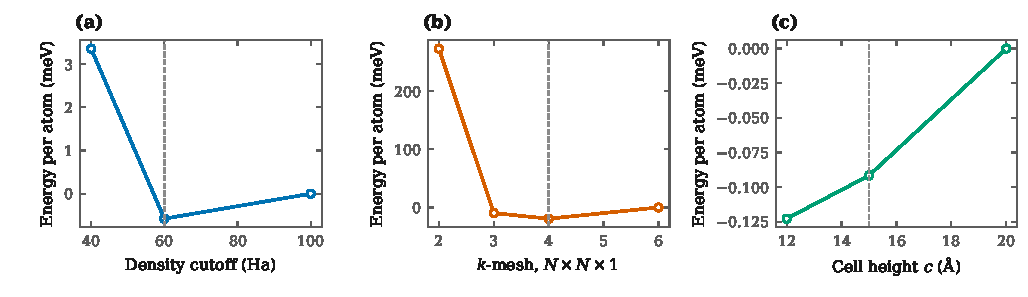
\includegraphics[width=\textwidth]{../figs/figS1.pdf}
\caption{Convergence for monolayer MoS$_2$. (a) Energy per atom against the
density-grid cutoff, referenced to 100~Ha. (b) Energy per atom against
$k$-point sampling, referenced to a $6\times6\times1$ mesh. (c) Energy per
atom against the cell height $c$, that is the repeat length along the axis
normal to the layer; the vacuum gap is $c$ less the layer thickness of about
3.1~\AA. Dashed lines mark the production settings.}
\label{figS1}
\end{figure*}

\emph{Strain sweep and elastic constants.} The in-plane lattice constant is
scaled by $1+\varepsilon$ with $\varepsilon\in\{-2,-1,0,+1,+2\}\%$, and the
chalcogen height by $1-\nu_\perp\varepsilon$ with $\nu_\perp=0.25$; the
chalcogen height at zero strain is first relaxed by a three-point parabolic
scan. For an isotropic two-dimensional sheet under equal biaxial strain the
elastic energy density is $u=(C_{11}+C_{12})\varepsilon^2$, so
\begin{equation}
C_{11}+C_{12}=\frac{1}{2A_0}\frac{\mathrm{d}^2E}{\mathrm{d}\varepsilon^2},
\end{equation}
with $A_0$ the cell area. We take $C_{12}\simeq0.25\,C_{11}$ to extract
$C_{11}$; this enters only the zone-edge acoustic frequency estimate.

Because the zone-edge longitudinal acoustic frequency obeys
$\omega_{\rm LA}(M)\propto\sqrt{C_{11}}$ once the area scaling of the
Brillouin zone is included, its Gr\"uneisen parameter is
\begin{equation}
\gamma_{\rm LA}=-\tfrac12\,\frac{\mathrm{d}\ln C_{11}}{\mathrm{d}\ln A}.
\label{eq:glaS}
\end{equation}
We evaluate this without ambiguity by fitting a local three-point quadratic to
$E(\varepsilon)$ centred at $\varepsilon=\pm1\%$, dividing by the strained
cell area at that point, and differencing the logarithms. For MoS$_2$ this
gives $\gamma_{\rm LA}=\GammaLA$. Section~\ref{sec:sep} shows that the edge
assignment is independent of this value.

\emph{Frozen phonons.} The two Raman-active zone-centre modes are obtained by
symmetry-adapted displacements. For the in-plane $E'$ mode the metal and the
chalcogen pair move oppositely with zero net momentum, $m_Mu_M=-2m_Xu_X$, so
the mass-weighted normal coordinate satisfies $Q^2=2m_Xu_X^2(1+2m_X/m_M)$,
and the force constant is taken from the symmetric second difference
\begin{equation}
\omega^2=\frac{E(+u)+E(-u)-2E(0)}{Q^2},
\label{eq:sym}
\end{equation}
with $u=0.05$~\AA. Using both signs matters because the chalcogen height is
relaxed only at zero strain, so at finite strain the structure carries a small
residual force along the mode coordinate, and a one-sided difference would
alias that force into the extracted Gr\"uneisen parameter.

The $A_1'$ mode is handled differently, and more directly. Its normal
coordinate is the chalcogen half-thickness itself, with $Q^2=2m_Xz^2$, so a
three-point parabolic scan of that single coordinate returns both the relaxed
geometry, from the position of the minimum, and the force constant, from the
curvature there. Evaluating the curvature at the relaxed point removes the
residual-force problem altogether, so this is the route used for every
$\omega_{A_1'}$ and $\gamma_{A_1'}$ reported here, with a scan half-width of
0.04~\AA. The harmonic assumption is checked by repeating the MoS$_2$
symmetric-displacement calculation at $u=0.025$, 0.05 and $0.075$~\AA, over
which $\omega_{A_1'}$ moves by 0.5~cm$^{-1}$.

Repeating at $\varepsilon=\pm1\%$ gives the mode Gr\"uneisen parameters,
$\gamma_i=-(1/2\omega_i)\,\mathrm{d}\omega_i/\mathrm{d}\varepsilon$, where the
factor of two converts linear biaxial strain to areal strain.
Figure~\ref{figS2} shows the underlying energy curves and compares the
computed zone-centre frequencies with experiment; Table~\ref{tab:dft}
collects the constants. Measured mode Gr\"uneisen parameters across the full
resonant Raman band set of MoS$_2$ are available for
comparison.\cite{Gontijo2025} Absolute frequencies carry
the usual few-percent PBE error, so the forward model uses measured
zone-centre frequencies as the anchor\cite{Mignuzzi2015,Berkdemir2013,Terrones2014}
and the computed Gr\"uneisen parameters as the strain response.

\begin{figure*}[!tb]
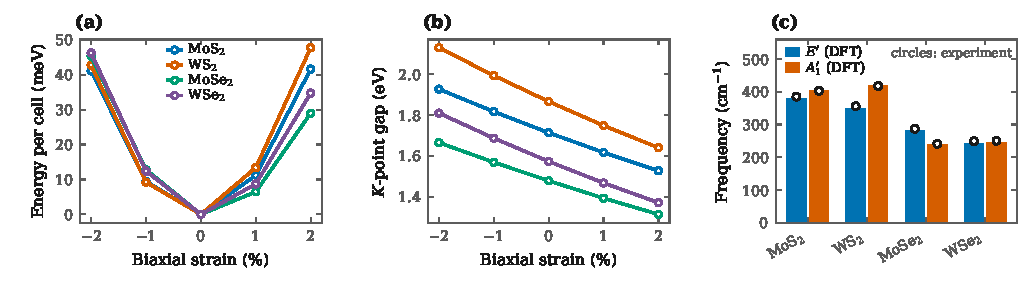
\includegraphics[width=\textwidth]{../figs/figS2.pdf}
\caption{(a) Total energy against biaxial strain, referenced to zero strain.
(b) $K$-point gap against biaxial strain. (c) Frozen-phonon zone-centre
frequencies compared with measured values.}
\label{figS2}
\end{figure*}

\begin{table*}[t]
\caption{First-principles constants computed in this work. $a_0$ is the
in-plane lattice constant used (\AA), $\omega_{E'}$ and $\omega_{A_1'}$ are the
frozen-phonon zone-centre frequencies (cm$^{-1}$), $\gamma_{E'}$ and
$\gamma_{A_1'}$ the corresponding mode Gr\"uneisen parameters,
$\gamma_{\rm LA}$ the acoustic Gr\"uneisen parameter obtained from the strain
dependence of the elastic constant, and $C_{2D}$ the in-plane elastic constant
(N/m).  The lattice constant is an input; every other entry is computed in
this work and none is fitted.}
\label{tab:dft}
\begin{ruledtabular}
\begin{tabular}{lccccccc}
Material & $a_0$ & $\omega_{E'}$ & $\omega_{A_1'}$ & $\gamma_{E'}$ &
$\gamma_{A_1'}$ & $\gamma_{\rm LA}$ & $C_{2D}$ \\
\hline
MoS$_2$ & 3.184 & 380 & 405 & 1.01 & 0.63 & 2.30 & 151 \\
WS$_2$ & 3.183 & 350 & 418 & 1.05 & 0.65 & 2.34 & 165 \\
MoSe$_2$ & 3.319 & 281 & 237 & 1.00 & 0.66 & 3.07 & 124 \\
WSe$_2$ & 3.322 & 243 & 245 & 1.07 & 0.68 & 3.15 & 135 \\
\end{tabular}
\end{ruledtabular}
\end{table*}

\begin{table*}[t]
\caption{Inversion of the published atomic-layer-deposited and sputtered
MoS$_2$ films. $R_{\rm sh}$ and $R_{\rm LA}$ are the two disorder-activated
Raman ratios, $n_{\rm d}$ (cm$^{-2}$) and $L_{\rm D}$ (nm) the inverted defect
density and mean inter-defect distance, and the last two columns the measured
and point-defect-limited mobility (cm$^2$V$^{-1}$s$^{-1}$).}
\label{tab:nattoo}
\begin{ruledtabular}
\begin{tabular}{lcccccc}
Film & $R_{\rm sh}$ & $R_{\rm LA}$ & $n_{\rm d}$ & $L_{\rm D}$ &
$\mu_{\rm meas}$ & $\mu_{\rm ceiling}$ \\
\hline
ALD as-grown & 0.325 & 0.043 & $7.3\times10^{12}$ & 3.7 & 0.16 & 29 \\
ALD annealed & 0.230 & 0.032 & $5.4\times10^{12}$ & 4.3 & 0.44 & 33 \\
sputtered as-grown & 0.687 & 0.128 & $2.2\times10^{13}$ & 2.1 & 0.03 & 14 \\
sputtered annealed & 0.507 & 0.087 & $1.5\times10^{13}$ & 2.6 & --- & 19 \\
\end{tabular}
\end{ruledtabular}
\end{table*}

\begin{table*}[t]
\caption{Provenance of every group of constants used in this work.  Entries
marked ``this work'' are computed here from first principles; ``calibrated
once'' means the value was fixed a single time against the cited published
result and then held for every number reported; ``geometry'' means a nominal
device dimension; ``assumed'' marks a modelling choice stated in the text; and
``not used'' marks a constant that is present in the code but multiplies zero
in every result reported here.}
\label{tab:prov}
\begin{ruledtabular}
\begin{tabular}{@{}>{\raggedright\arraybackslash}p{0.26\textwidth} l
>{\raggedright\arraybackslash}p{0.44\textwidth}@{}}
Constants & Origin & Source \\
\hline
BANDS & literature & Jin et al., Phys. Rev. B 90, 045422 (2014) \\
MU\_PHONON & literature & Jin et al., Phys. Rev. B 90, 045422 (2014) \\
PHONON & literature & Mignuzzi 2015, Berkdemir 2013, Terrones 2014 \\
EXCITON & literature & Henriquez-Guerra et al., ACS AMI 15, 57369 (2023) \\
DOPING\_MoS2 & literature & Chakraborty et al., Phys. Rev. B 85, 161403 (2012) \\
RAMAN\_CAL & literature & Mignuzzi et al., Phys. Rev. B 91, 195411 (2015) \\
gamma\_E, gamma\_A, gamma\_LA, C2D, dgap\_deps & this work & frozen phonons and biaxial strain sweep, this work \\
C\_A (WS2, MoSe2, WSe2) & this work & predicted in this work by transfer \\
GAMMA\_MEAS & literature & Michail et al., ACS AMI 16, 49602 (2024), MoS2 and WSe2 only \\
CHI\_DOP & literature & Chernikov et al., Phys. Rev. Lett. 115, 126802 (2015) \\
DEQK\_DEPS, DEGK\_DEPS & not used & strain-tuned valley shift, zero strain in every reported result \\
COX, STACK & geometry & nominal gate-stack capacitance and permittivity \\
VSAT & literature & Smithe et al., Nano Lett. 18, 4516 (2018), MoS2 value used for all four \\
P\_SPEC & assumed & fully diffuse etched edge, p = 0 \\
halo\_contrast & assumed & 20x defect density inside the damage halo \\
Udef & calibrated once & fixed once on Dossena et al., npj 2D Mater. Appl. 9, 67 (2025) \\
N\_IT & calibrated once & fixed once on measured monolayer field-effect mobility \\
\end{tabular}
\end{ruledtabular}
\end{table*}


\section{Separating charge from strain}
\label{sec:sep}

The two observables are the shifts of the first-order $A_1'$ mode and of the
disorder-activated 2LA(M) overtone relative to an unperturbed reference,
\begin{equation}
\begin{pmatrix}\Delta\omega_{A_1'}\\[2pt]\Delta\omega_{2\rm LA}\end{pmatrix}
=\begin{pmatrix}
-2\gamma_{A_1'}\omega_{A_1'}^0/100 & \lambda_{A_1'}\\[2pt]
-2\gamma_{\rm LA}\,\omega_{2\rm LA}^0/100 & 0
\end{pmatrix}
\begin{pmatrix}\varepsilon\\ n\end{pmatrix},
\label{eq:2x2}
\end{equation}
with $\varepsilon$ in percent and $n$ in units of $10^{13}$~cm$^{-2}$. The
zero in the lower right is the physical content of the method. The
renormalisation of the out-of-plane optical mode is a measured, symmetry
selective coupling to the $K$-valley electron
density;\cite{Chakraborty2012} the corresponding coefficient for the zone-edge
acoustic overtone has not been measured, and setting it to zero is an
assumption, not a citation. It is bounded below rather than asserted. The
system is solved as a regularised least squares problem with measurement standard deviations of 0.15 and
0.30~cm$^{-1}$ on the two channels and a broad prior, and the reported error
bars are the square roots of the diagonal of the posterior covariance.

Because $\Delta\omega_{2\rm LA}=0$ at the ribbon edge within the measurement
uncertainty, the second row of Eq.~(\ref{eq:2x2}) pins $\varepsilon$ near zero
for \emph{any} non-zero value of $\gamma_{\rm LA}$, and the entire $A_1'$
shift is carried by the second column. This is why the recovered edge charge
in Fig.~3(a) of the main text is flat across the whole scanned range of
$\gamma_{\rm LA}$: the spread is \EdgeNspread\%\ over
$0.4\le\gamma_{\rm LA}\le2.6$, a range that brackets the plausible values for
MoS$_2$ shaded in that panel. Only the interior inhomogeneity, where the
overtone does shift, depends on $\gamma_{\rm LA}$. For the same reason the
recovered edge charge is independent of $\gamma_{A_1'}$: with
$\varepsilon$ pinned at zero the first row of Eq.~(\ref{eq:2x2}) reduces to
$n=\Delta\omega_{A_1'}/\lambda_{A_1'}$. Adopting the measured optical
Gr\"uneisen parameter of MoS$_2$, $\gamma_{A_1'}=0.31$, in place of the
calculated \gAdftMoSTwo\ therefore leaves the edge density unchanged to four
significant figures, and leaves the interior strain unchanged as well, because
that is pinned by the 2LA(M) row, which contains no $\gamma_{A_1'}$. What it
does change is the small residual charge assigned to the interior spot, which
is consistent with zero either way.

A second assumption is that the overtone does not renormalise with carrier
density. No gated measurement of that coefficient exists, so we bound it
rather than assume it: setting $\lambda_{2\rm LA}$ to a fraction of the $A_1'$
coefficient scaled by the frequency ratio and repeating the solve, a fraction
of one half changes the recovered edge density by \OvertoneBound\%.

The dominant systematic uncertainty is therefore neither $\gamma_{\rm LA}$ nor
$\lambda_{2\rm LA}$ but the $A_1'$ doping coefficient
$\lambda_{A_1'}=-2.2$~cm$^{-1}$ per $10^{13}$~cm$^{-2}$, a measured quantity
with roughly 15\% uncertainty, to which the recovered density is inversely
proportional. The second is the edge width $w_{\rm e}$ used to convert an
areal to a line density. Tip-enhanced Raman resolves about 10~nm and
nano-optical studies place the electronic edge region of MoS$_2$ between about
5 and 20~nm,\cite{Su2019,Wu2016} so we take $w_{\rm e}=\Wedge$~nm. The excess
areal density $n$ becomes a line density
$\sigma_{\rm e}=n\,w_{\rm e}$ along each edge, which is the quantity that
enters Eq.~(1) of the main text; varying $w_{\rm e}$ over the range above moves
the critical width on the high-$\kappa$ stack from \WcHfOwFive\ to
\WcHfOwTwenty~nm and leaves the halo-limited branch unchanged.

Finally, the sign of the edge charge is environment dependent. The ribbons
measured by tip-enhanced Raman were supported on gold, which donates
electrons; nano-optical measurements of MoS$_2$ edges on oxide instead report
local depletion.\cite{Su2019,Sousa2024} Only the magnitude is transferred to
the electrostatic analysis.

\section{Transport and nanoribbon model}
\label{sec:transport}

\emph{Scattering channels.} The wide-channel mobility combines three channels
by Matthiessen's rule. The phonon-limited value is the published
first-principles $K$-valley-dominated mobility.\cite{Jin2014} Neutral point
defects are treated as short-range scatterers, for which the
two-dimensional Fermi golden rule gives an energy-independent rate,
\begin{equation}
\frac{1}{\tau_{\rm pd}}=\frac{m^*n_{\rm d}U^2}{\hbar^3},\qquad
\mu_{\rm pd}=\frac{e\hbar^3}{m^{*2}n_{\rm d}U^2},
\end{equation}
with $U$ the areal integral of the defect potential. Charge at the dielectric
interface is treated with a screened two-dimensional Coulomb potential,
$V(q)=e^2\exp(-2qd)/[2\epsilon_0\epsilon_{\rm env}(q+q_{\rm s})]$ with the
Thomas-Fermi wavevector
$q_{\rm s}=m^*e^2/(2\pi\epsilon_0\epsilon_{\rm env}\hbar^2)$, a setback
$d=0.3$~nm representing the van der Waals gap, and
\begin{equation}
\frac{1}{\tau_{\rm ci}}=\frac{m^*n_{\rm it}}{2\pi\hbar^3}
\int_0^{2\pi}|V(q)|^2\left(1-\cos\theta\right)\mathrm{d}\theta ,
\end{equation}
with $q=2k_{\rm F}\sin(\theta/2)$. Figure~\ref{fig:transport}(a) shows the
decomposition, and Fig.~\ref{fig:transport}(b) the width dependence of the ribbon
mobility for four halo widths. Two constants are calibrated once and then held for every
result: $U=\Udefect$~eV\,nm$^2$, fixed against the first-principles quantum
transport result for disordered WS$_2$,\cite{Dossena2025} and the interface
charge density $n_{\rm it}$ of each gate stack, fixed against the measured
field-effect mobility of a clean monolayer on SiO$_2$ and the measured
wide-channel on-current on the high-$\kappa$ stack. Everything else is
computed or taken from a published measurement, as listed in
Table~\ref{tab:prov}.

\emph{Nanoribbon layer.} Three effects are added. Diffuse edge scattering in
the two-dimensional Fuchs-Sondheimer limit gives
$\mu_{\rm edge}=eW/(m^*\bar v)$ with $\bar v=\sqrt{\pi k_{\rm B}T/2m^*}$; at
the widths of interest this channel is weak, consistent with the measured
absence of mobility degradation from 850 down to 75~nm.\cite{Pena2026} The
patterning damage halo is treated as two parallel conductors,
\begin{equation}
\mu(W)=\frac{(W-2w_{\rm h})\mu_{\rm int}+2w_{\rm h}\mu_{\rm dam}}{W},
\end{equation}
with $\mu_{\rm int}$ and $\mu_{\rm dam}$ evaluated at the bulk and elevated
defect densities. Fixed edge charge shifts the threshold by
Eq.~(1) of the main text, reducing the gate overdrive, and the drain current
per unit width follows from
\begin{equation}
\frac{I_{\rm on}}{W}=qn_{\rm s}\frac{\mu\mathcal{E}}
{1+\mu\mathcal{E}/v_{\rm sat}},\qquad
n_{\rm s}=\frac{C_{\rm ox}(V_{\rm ov}-\Delta V_{\rm T})}{q},
\label{eq:ion}
\end{equation}
with $\mathcal{E}=V_{\rm DS}/L_{\rm ch}$. Reported results use
$V_{\rm ov}=\Vov$~V, $V_{\rm DS}=1$~V and $L_{\rm ch}=300$~nm, matching the
measured devices, and the measured monolayer MoS$_2$ saturation velocity
$v_{\rm sat}=3.4\times10^{6}$~cm/s.\cite{Smithe2018} No comparable
measurement exists for WS$_2$, MoSe$_2$ or WSe$_2$, so the same value is used
for all four rather than a guessed material dependence. The critical width $W_{\rm c}$ is the width at which
$I_{\rm on}/W$ falls to half of its wide-channel value at the stated gate
overdrive; Fig.~\ref{fig:transport}(c) shows that it grows smoothly, by a
factor of 3.8 for a 5~nm halo and by 2.4 for a 150~nm halo,
as the criterion is tightened from 0.3 to 0.8, with the ordering of the halo
widths unchanged, so the choice of 0.5 fixes the scale of $W_{\rm c}$ but not
the comparisons drawn from it. Because the edge-charge
term enters through $V_{\rm ov}-\Delta V_{\rm T}$, that branch of $W_{\rm c}$
scales inversely with $V_{\rm ov}$, whereas the halo branch does not; the two
contributions are therefore reported separately in the main text.

\begin{figure*}[!tb]
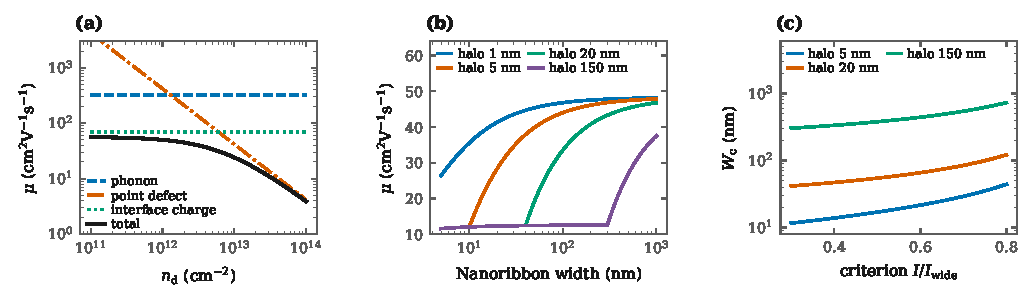
\includegraphics[width=\textwidth]{../figs/figS3.pdf}
\caption{(a) Decomposition of the MoS$_2$ sheet mobility into its three
scattering channels. (b) Ribbon mobility against width for four damage-halo
widths. (c) Sensitivity of the critical width to the choice of criterion.
(d) The compact expression of Eq.~(\ref{eq:ion}) against the self-consistent
solve of Eqs.~(\ref{eq:gate}) to (\ref{eq:cont}); the two differ by a nearly
constant factor, so the critical width, which is a ratio, is almost unchanged.}
\label{fig:transport}
\end{figure*}

\section{Self-consistent device solve}
\label{sec:device}

Every current that the article compares with measurement comes from a
self-consistent solve of the channel rather than from the compact expression of
Eq.~(\ref{eq:ion}); the design map and growth-technology lines of Fig.~4(b),
the four-material screening of Fig.~4(c) and the critical-width scans use the
compact expression, which is validated against the self-consistent solve at the
end of this section. Two fields are carried at each point along the channel:
the surface band bending $\psi$, that is the local shift of the conduction band
edge with respect to the source Fermi level, and the electron quasi-Fermi
potential $V$. They satisfy the vertical electrostatic balance
\begin{equation}
C_{\rm ox}(V_{\rm ov}-\Delta V_{\rm T}-\psi)=qn_{\rm s}(\psi,V),
\label{eq:gate}
\end{equation}
with the sheet density of a two-dimensional parabolic band,
\begin{equation}
n_{\rm s}=g_{\rm 2D}k_{\rm B}T
\ln\!\left[1+e^{\,q(\psi-V)/k_{\rm B}T}\right],\qquad
g_{\rm 2D}=\frac{g_{\rm s}g_{\rm v}m^{*}}{2\pi\hbar^{2}},
\label{eq:ns}
\end{equation}
and current continuity for drift and diffusion,
\begin{equation}
\frac{\mathrm{d}}{\mathrm{d}x}
\left[\frac{qn_{\rm s}\mu\,\mathrm{d}V/\mathrm{d}x}
{1+(\mu/v_{\rm sat})|\mathrm{d}V/\mathrm{d}x|}\right]=0 .
\label{eq:cont}
\end{equation}
Writing the charge as Eq.~(\ref{eq:ns}) rather than as
$C_{\rm ox}(V_{\rm GS}-V_{\rm T})/q$ places the quantum capacitance
$C_{\rm q}=q^{2}g_{\rm 2D}f(\eta)$ in series with the oxide. The valley
degeneracy is $g_{\rm v}=2$ for the two $K$ valleys of both bands. The spin
degeneracy is $g_{\rm s}=2$ for electrons, whose conduction-band spin-orbit
splitting at $K$ is a few tens of meV, and $g_{\rm s}=1$ for holes, whose
valence-band splitting is several hundred meV, so that only the upper spin
branch is occupied at the densities of interest.\cite{Kormanyos2015} For MoS$_2$ on the
high-$\kappa$ stack $C_{\rm q}=\ScCq~\mu$F/cm$^{2}$, so the series combination
removes \ScCqCorr\%\ of the charge that the oxide alone would imply.

Because $V$ is the quasi-Fermi potential, drift and diffusion are both carried
by its gradient, and the fall of $n_{\rm s}$ towards the drain that the compact
expression omits appears automatically. The two equations are assembled on a
one-dimensional finite-volume mesh and solved together by Newton's method in
DEVSIM, an open-source device simulator, with the Jacobian formed from the
symbolic derivatives of the models.\cite{Sanchez2022} The contact resistance is
closed by bisection on the internal drain bias: the channel current is monotone
in that bias, so $g(v)=v+2I(v)R_{\rm c}-V_{\rm DS}$ has a single root, with $R_{\rm c}$
quoted per contact, whereas a
fixed point on the current diverges once the contact carries most of the
applied bias, which is exactly the p-type regime of interest.

Four checks run with the code. The band bending returned by the coupled Newton
solve matches an independent bisection solution of Eq.~(\ref{eq:gate}) at every
node to $\ScPsiErr$, using only the converged quasi-Fermi potential as input;
the residual of Eq.~(\ref{eq:gate}) itself, measured against the gate charge
$C_{\rm ox}V_{\rm ov}$, is $\ScElecErr$; the current entering the source equals
the current leaving the drain to $\ScContErr$; and in the long-channel,
low-field limit the solver reproduces the textbook square law to
\ScSquareErr\%\ once $C_{\rm q}$ is placed in series with the oxide, while the
uncorrected square law is high by the \ScCqCorr\%\ quoted above.

Figure~\ref{fig:transport}(d) compares the two models over the whole width
range. The compact expression is high by a nearly constant factor: the ratio of
the self-consistent to the compact current is $\ScRatio$ with a spread of
$\ScRatioSpread$ for $W>12$~nm, close to the triode factor
$(V_{\rm ov}-V_{\rm DS}/2)/V_{\rm ov}=0.67$ that the compact form leaves out.
Because the critical width is defined as a ratio of currents, that common
factor cancels almost entirely: $W_{\rm c}=\WcSelfCons$~nm from the
self-consistent solve against \WcCompact~nm from the compact expression, a
difference of \WcModelDiff\%. Every conclusion in the article about how narrow a
ribbon can usefully be made therefore rests on a quantity that the two models
agree on, while the absolute currents compared with measurement are the
self-consistent ones.

\section{Physics-guided adjoint inversion}
\label{sec:adjoint}

The disorder-activated intensity ratio and the A-exciton energy add two
further observables, so that a full hyperspectral acquisition constrains the
three-component latent state
$\bm\theta=(\log_{10}n_{\rm d},\varepsilon,n)$ through
\begin{align}
\omega_i &= \omega_i^0(1-2\gamma_i\varepsilon/100)+\lambda_in,
\quad i\in\{E',A_1'\},\\
R_{\rm A} &= C_{\rm A}n_{\rm d}\times10^{-14},\\
E_{\rm A} &= E_{\rm A}^0+\Xi\varepsilon/1000+\chi n/1000 .
\end{align}
Here $\chi$ is the shift of the A-exciton resonance with electron density, for
which we take the scale reported for electrostatically gated monolayer
WS$_2$,\cite{Chernikov2015} where screening of the exciton binding energy
outweighs the bandgap renormalisation. This coefficient enters only the
three-field image inversion demonstrated in this section; no result reported in
the main article depends on it. For an image we minimise
\begin{equation}
J=\tfrac12\sum_p\|\bm r_p\|^2_{C_{\rm d}^{-1}}
+\tfrac12\sum_p\|\Delta\bm\theta_p\|^2_{C_{\rm p}^{-1}}
+\tfrac12\sum_k\alpha_k\|\nabla\Theta_k\|^2 ,
\end{equation}
where the gradient-squared term encodes the expectation that the three fields
are continuous on the scale of the optical resolution and is what couples the
pixels. Because the forward operator is an explicit analytic chain, its
linearisation $G_p$ is available in closed form and the gradient is assembled
in one adjoint sweep,\cite{Plessix2006,Stuart2010}
\begin{equation}
\nabla_pJ=G_p^{\!\top}C_{\rm d}^{-1}\bm r_p
+C_{\rm p}^{-1}\Delta\bm\theta_p-\alpha_k\nabla^2\Theta_k\big|_p .
\end{equation}
The Gauss-Newton system is solved matrix free by conjugate gradients, so the
cost per iteration is one forward and one adjoint application regardless of
image size, and the posterior covariance follows from the Laplace
approximation $C_{\rm post}=(G^{\!\top}C_{\rm d}^{-1}G+C_{\rm p}^{-1})^{-1}$.

Three checks run automatically with the code. The analytic Jacobian matches a
central finite difference to a relative error of $\AdjJacErr$; the separately
implemented forward and adjoint applications satisfy
$\langle G\bm v,\bm w\rangle=\langle\bm v,G^{\!\top}\bm w\rangle$ to a
relative error of $\AdjDotErr$, that is to machine precision; and the assembled
map gradient matches a directional finite
difference of the full objective, regulariser included, to $\AdjMapErr$.

Figure~\ref{fig:adjoint} reports the conditioning and a synthetic recovery test on a
$48\times48$ pixel map containing a strained grain boundary, a doped patch and
a defective region. To avoid an inverse crime the data are generated with
coefficients that differ from those used in the inversion by three percent and
with heavy-tailed (Student $t$) noise, while the inversion assumes Gaussian
noise and the unperturbed coefficients. The objective stops decreasing after
\MapIter\ Gauss-Newton iterations out of the \MapIterMax\ requested, and the
solver separates the three fields with root-mean-square
errors of \RmseNd~dex, \RmseEps\%\ and $\RmseN\times10^{13}$~cm$^{-2}$.
Removing the intensity-ratio channel leaves the defect density on its prior,
which is why an intensity channel is indispensable. Note that the two frequency
channels of the image model are the two first-order modes $E'$ and $A_1'$: the
overtone used in Section~\ref{sec:sep} is a single-point observable and does
not enter here.

\begin{figure*}[!tb]
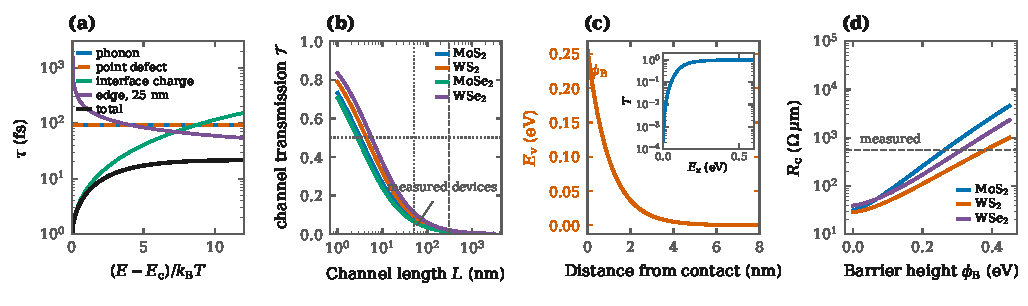
\includegraphics[width=\textwidth]{../figs/figS4.pdf}
\caption{Adjoint inversion. (a) Posterior correlation matrix. (b) Posterior
widths for three observable subsets. (c) Posterior widths against measurement
noise. (d) Objective decay of the matrix-free solver. (e)-(g) True and
recovered fields. (h) Recovery error distributions.}
\label{fig:adjoint}
\end{figure*}

\section{Inversion of published films}
\label{sec:published}

Table~\ref{tab:nattoo} lists the inverted state for the four
atomic-layer-deposited and sputtered MoS$_2$ films of
Ref.~\onlinecite{Nattoo2025}, obtained from
$I_{\rm LA}/I_{A_1'}=C_{\rm A}n_{\rm d}$ with the MoS$_2$ calibration
constant.\cite{Mignuzzi2015} Two disorder-activated ratios were measured
independently on the same films; if both are linear in $n_{\rm d}$ their ratio
must be constant, and we find $\NattooRatio\pm\NattooRatioSD$. The residual
scatter is systematic rather than random, the two deposition families
clustering at \NattooRatioALD\ and \NattooRatioSputt, which is expected
because the shoulder feature and the LA(M) peak have different resonance
conditions and the films differ in thickness. The detuning $\Delta$ that controls the transfer of $C_{\rm A}$ across the
family is itself observable: biaxial strain shifts the WS$_2$ B exciton and
measurably collapses the double-resonant 2LA(M) intensity, which is direct
evidence that the double-resonance picture used here is the right one for this
mode.\cite{Rodriguez2026} An independent calibration on
helium-ion irradiated material reports a larger
constant,\cite{Aryeetey2020} reflecting a different defect species; adopting
it would rescale all inverted defect densities by a common factor without
changing any relative conclusion. As a further check on the forward model, the
50~meV blue shift of the A exciton measured at a WS$_2$ grain boundary by
wide-field hyperspectral reflectance\cite{Peng2026} corresponds to
\GBstrain\%\ of compression when converted with the measured biaxial gauge
factor,\cite{Henriquez2023} against the \GBstrainRef\%\ quoted in the
original work with a bulk-like deformation potential.

The measured mobilities of these films fall between \DeficitLo\ and
\DeficitHi\ times below the point-defect ceiling. They are polycrystalline few-layer films whose electron
micrographs show vertical domains and grain
boundaries,\cite{Nattoo2025,vanderZande2013} so the deficit is expected and is
itself informative: it separates the point-defect contribution, which the
optical ratio measures, from the grain-boundary contribution, which it does
not.

\section{Limitations}

\begin{enumerate}
\item PBE without spin-orbit coupling. Absolute gaps and valley separations
carry the known functional spread, so published spin-orbit-resolved effective
masses are used\cite{Jin2014,Kormanyos2015} and only strain derivatives are
taken from our own calculations.
\item The edge charge is inferred from one published data set on one material,
and assumes the extracted density is uniform over an edge width of
\Wedge~nm.
\item The predicted calibration constants for WS$_2$, MoSe$_2$ and WSe$_2$
rest on a double-resonance scaling argument and have not been measured.
\item The model treats isolated point defects; grain-boundary networks and
dielectric disorder are not resolved, so the mobility ceiling is an upper
bound for nanocrystalline films.
\item The transport layer uses a constant relaxation time within each
scattering channel, so mobility is evaluated at a single carrier energy rather
than from a full energy-resolved integral. The device solve is semiclassical
drift and diffusion with a field-dependent velocity, so ballistic and
tunnelling transport are outside its scope, and the contact is represented by a
lumped series resistance rather than by a resolved Schottky barrier.
\item The comparison with the first-principles disordered WS$_2$
result\cite{Dossena2025} is good at $2\times10^{13}$~cm$^{-2}$
(\DosOnePred\ against \DosOneRef~cm$^2$V$^{-1}$s$^{-1}$) but the model
overestimates at $4\times10^{13}$~cm$^{-2}$ (\DosTwoPred\ against
\DosTwoRef), where the mean free path approaches the inter-defect spacing and
a semiclassical treatment is no longer adequate.
\end{enumerate}

\section{Data and code availability}

The archive of record is deposited at Zenodo,
\url{https://doi.org/10.5281/zenodo.21670316}.\cite{Mahim2026data} It holds the
raw PySCF output for every stage described in Section~\ref{sec:dft}, the
convergence and $k$-mesh cross-check runs, the reduced constants, every
digitised published measurement used in this work as a flat file with its
source stated in the header, the machine-readable results file behind every
number quoted here, and the figures as published.

The development repository is
\url{https://github.com/Tanvir-Mahmud-Mahim/Width-scaling-in-monolayer-semiconductor-nanoribbon-transistors}.
\texttt{dft/} contains the PySCF drivers and the post-processing that reduces
raw output to the constants used by the models; \texttt{rapid/} contains the
parameter table with a provenance tag on every entry, the forward model and its
analytic Jacobian, the adjoint solvers and their three verification tests, the
transport and nanoribbon layers, the published data sets with their sources,
and the scripts that regenerate every number, figure and table. Running
\texttt{python -m rapid.analysis}, then \texttt{rapid.figures},
\texttt{rapid.supplement} and \texttt{rapid.numbers} reproduces the article end
to end from the stored first-principles output; re-running the density
functional theory requires only PySCF and takes a few hours on two cores.

\nocite{aip41Control}
\bibliographystyle{aipnum4-1}
\bibliography{refs}

\end{document}
